\documentclass[mathserif]{beamer}
\usetheme{Dresden}
\usepackage{moreverb}
% math stuff
\usepackage{tikz}
\usepackage{amsmath}
\usepackage{amsfonts}
\usepackage{amsthm}
\usepackage{amssymb}
\usepackage{cancel}
% code stuff
\usepackage{verbatim}
%% stuff needed for pygments code
\usepackage{fancyvrb}
\usepackage{color}
\usepackage{mathtools}
% font stuff
\usepackage[T1]{fontenc}
\usepackage[sc]{mathpazo}

% beamer specific things.
\setbeamertemplate{navigation symbols}{} %no navigation symbols.
\title[Stabilization of POD-ROMs]{Stabilization of POD-ROMs}

\author[David Wells]{David Wells}
\institute{Virginia Tech/Rensselaer Polytechnic Institute}
\date{Wednesday, August 5, 2015}

% vector notation
\newcommand{\va}{\vec{a}}
\newcommand{\bb}{\vec{b}}
\newcommand{\cc}{\vec{c}}
\newcommand{\ff}{\vec{f}}
\newcommand{\nn}{\vec{n}}
\newcommand{\uu}{\vec{u}}
\newcommand{\ww}{\vec{w}}
\newcommand{\xx}{\vec{x}}
\newcommand{\twoVector}[2]{\begin{bmatrix} #1 \\ #2 \end{bmatrix}}
\newcommand{\threeVector}[3]{\begin{bmatrix} #1 \\ #2 \\ #3 \end{bmatrix}}
\newcommand{\twoVectorT}[2]{\begin{bmatrix} #1 & #2 \end{bmatrix}}
\newcommand{\threeVectorT}[3]{\begin{bmatrix} #1 & #2 & #3 \end{bmatrix}}
\newcommand{\fourVectorT}[4]{\begin{bmatrix} #1 & #2 & #3 & #4 \end{bmatrix}}
\newcommand{\vr}{\vec{v}_r}

% bold commands
\newcommand{\bx}{{\mathbf x}}
\newcommand{\by}{{\mathbf y}}

% integral notation
\newcommand{\dxx}{\,d\xx}
\newcommand{\dll}{\,d\vec{l}}
\newcommand{\intO}{\int_\Omega}

\newcommand{\sumT}{\sum_{T\in \mathcal{T}_h}}
\newcommand{\intT}{\int_T}
\newcommand{\Th}{\mathcal{T}_h}

% typesetting
\newcommand{\todo}[1]{{\color{red}#1}}
\newcommand{\eg}{e.g., }
\newcommand{\ie}{i.e., }
\newcommand{\frameBoxShort}[1]{\begin{center} \begin{minipage}{0.8\textwidth}\begin{center}\fbox{#1}\end{center}\end{minipage} \end{center}}
\newcommand{\frameBox}[1]{\noindent\begin{center} \begin{minipage}{\textwidth}\framebox{#1}\end{minipage} \end{center}}

% SUPG notation
\newcommand{\eps}{\varepsilon}
\newcommand{\SDNorm}[1]{||| #1 |||_{SD}}
\newcommand{\SDRNorm}[1]{||| #1 |||_{\mathrm{SUPG}, r}}
\newcommand{\SDInner}[2]{a(#1, #2)_{SD}}
\newcommand{\SUPGRInner}[1]{a(#1)_{\mathrm{SUPG}, r}}
\newcommand{\half}{1/2}
\newcommand{\threehalves}{3/2}

% functional analysis
\newcommand{\abs}[1]{\ensuremath{\left| #1 \right|}}
\newcommand{\Norm}[1]{\ensuremath{\| #1 \|}}
\newcommand{\Norms}[1]{\ensuremath{\left\| #1 \right\|}}
\newcommand{\Seminorm}[1]{\ensuremath{| #1 |}}
\newcommand{\Seminorms}[1]{\ensuremath{\left| #1 \right|}}
\newcommand{\Langles}[1]{\left\langle#1\right\rangle}
\newcommand{\Brackets}[1]{\ensuremath{\left\{#1\right\}}}

% POD notation
\newcommand{\snapsum}{\sum_{n = 0}^{R - 1}} % sum of snapshots
\newcommand{\remainder}[1]{\sum_{#1 = r}^{R - 1}} % sum from r to R - 1
\newcommand{\podsum}[1]{\sum_{#1 = 0}^{r - 1}} % sum of POD vectors
% (uh(., tl), phij(.))
\newcommand{\inl}[1]{\Langles{u_n, \phi_{#1}}}
\newcommand{\podvec}{\vec{\varphi}}
\newcommand{\OO}{\mathcal{O}}

% NS notation
\newcommand{\reinv}{\dfrac{1}{Re}}

% NS and POD notation
\newcommand{\usteady}{\uu_s}
\newcommand{\podgalerkin}{\usteady + \podsum{j} a_j(t) \podvec_j(\xx)}
\newcommand{\podgalerkinx}{\uu_{s0} + \podsum{j} a_j(t) \varphi_{j0}(\xx)}

\newcommand{\evaluateBetween}[2]{\, \biggr\rvert_{#1}^{#2}}
\newcommand{\RR}{\mathbb{R}}
\newcommand{\mult}{\dfrac{1}{(2 \pi)^{n/2}}}
\newcommand{\multt}{\dfrac{1}{\sqrt{2 \pi}}}

% filtering notation
\newcommand{\FF}{\mathcal{F}}

\makeatletter
\def\PY@reset{\let\PY@it=\relax \let\PY@bf=\relax%
    \let\PY@ul=\relax \let\PY@tc=\relax%
    \let\PY@bc=\relax \let\PY@ff=\relax}
\def\PY@tok#1{\csname PY@tok@#1\endcsname}
\def\PY@toks#1+{\ifx\relax#1\empty\else%
    \PY@tok{#1}\expandafter\PY@toks\fi}
\def\PY@do#1{\PY@bc{\PY@tc{\PY@ul{%
    \PY@it{\PY@bf{\PY@ff{#1}}}}}}}
\def\PY#1#2{\PY@reset\PY@toks#1+\relax+\PY@do{#2}}

\expandafter\def\csname PY@tok@ow\endcsname{\let\PY@bf=\textbf\def\PY@tc##1{\textcolor[rgb]{0.67,0.13,1.00}{##1}}}
\expandafter\def\csname PY@tok@gr\endcsname{\def\PY@tc##1{\textcolor[rgb]{1.00,0.00,0.00}{##1}}}
\expandafter\def\csname PY@tok@vg\endcsname{\def\PY@tc##1{\textcolor[rgb]{0.10,0.09,0.49}{##1}}}
\expandafter\def\csname PY@tok@cm\endcsname{\let\PY@it=\textit\def\PY@tc##1{\textcolor[rgb]{0.25,0.50,0.50}{##1}}}
\expandafter\def\csname PY@tok@s1\endcsname{\def\PY@tc##1{\textcolor[rgb]{0.73,0.13,0.13}{##1}}}
\expandafter\def\csname PY@tok@o\endcsname{\def\PY@tc##1{\textcolor[rgb]{0.40,0.40,0.40}{##1}}}
\expandafter\def\csname PY@tok@na\endcsname{\def\PY@tc##1{\textcolor[rgb]{0.49,0.56,0.16}{##1}}}
\expandafter\def\csname PY@tok@err\endcsname{\def\PY@bc##1{\setlength{\fboxsep}{0pt}\fcolorbox[rgb]{1.00,0.00,0.00}{1,1,1}{\strut ##1}}}
\expandafter\def\csname PY@tok@mo\endcsname{\def\PY@tc##1{\textcolor[rgb]{0.40,0.40,0.40}{##1}}}
\expandafter\def\csname PY@tok@cp\endcsname{\def\PY@tc##1{\textcolor[rgb]{0.74,0.48,0.00}{##1}}}
\expandafter\def\csname PY@tok@kn\endcsname{\let\PY@bf=\textbf\def\PY@tc##1{\textcolor[rgb]{0.00,0.50,0.00}{##1}}}
\expandafter\def\csname PY@tok@gi\endcsname{\def\PY@tc##1{\textcolor[rgb]{0.00,0.63,0.00}{##1}}}
\expandafter\def\csname PY@tok@nn\endcsname{\let\PY@bf=\textbf\def\PY@tc##1{\textcolor[rgb]{0.00,0.00,1.00}{##1}}}
\expandafter\def\csname PY@tok@go\endcsname{\def\PY@tc##1{\textcolor[rgb]{0.53,0.53,0.53}{##1}}}
\expandafter\def\csname PY@tok@mf\endcsname{\def\PY@tc##1{\textcolor[rgb]{0.40,0.40,0.40}{##1}}}
\expandafter\def\csname PY@tok@bp\endcsname{\def\PY@tc##1{\textcolor[rgb]{0.00,0.50,0.00}{##1}}}
\expandafter\def\csname PY@tok@vc\endcsname{\def\PY@tc##1{\textcolor[rgb]{0.10,0.09,0.49}{##1}}}
\expandafter\def\csname PY@tok@ne\endcsname{\let\PY@bf=\textbf\def\PY@tc##1{\textcolor[rgb]{0.82,0.25,0.23}{##1}}}
\expandafter\def\csname PY@tok@nl\endcsname{\def\PY@tc##1{\textcolor[rgb]{0.63,0.63,0.00}{##1}}}
\expandafter\def\csname PY@tok@gh\endcsname{\let\PY@bf=\textbf\def\PY@tc##1{\textcolor[rgb]{0.00,0.00,0.50}{##1}}}
\expandafter\def\csname PY@tok@vi\endcsname{\def\PY@tc##1{\textcolor[rgb]{0.10,0.09,0.49}{##1}}}
\expandafter\def\csname PY@tok@il\endcsname{\def\PY@tc##1{\textcolor[rgb]{0.40,0.40,0.40}{##1}}}
\expandafter\def\csname PY@tok@mb\endcsname{\def\PY@tc##1{\textcolor[rgb]{0.40,0.40,0.40}{##1}}}
\expandafter\def\csname PY@tok@kr\endcsname{\let\PY@bf=\textbf\def\PY@tc##1{\textcolor[rgb]{0.00,0.50,0.00}{##1}}}
\expandafter\def\csname PY@tok@c1\endcsname{\let\PY@it=\textit\def\PY@tc##1{\textcolor[rgb]{0.25,0.50,0.50}{##1}}}
\expandafter\def\csname PY@tok@nc\endcsname{\let\PY@bf=\textbf\def\PY@tc##1{\textcolor[rgb]{0.00,0.00,1.00}{##1}}}
\expandafter\def\csname PY@tok@mh\endcsname{\def\PY@tc##1{\textcolor[rgb]{0.40,0.40,0.40}{##1}}}
\expandafter\def\csname PY@tok@sc\endcsname{\def\PY@tc##1{\textcolor[rgb]{0.73,0.13,0.13}{##1}}}
\expandafter\def\csname PY@tok@sb\endcsname{\def\PY@tc##1{\textcolor[rgb]{0.73,0.13,0.13}{##1}}}
\expandafter\def\csname PY@tok@nt\endcsname{\let\PY@bf=\textbf\def\PY@tc##1{\textcolor[rgb]{0.00,0.50,0.00}{##1}}}
\expandafter\def\csname PY@tok@ge\endcsname{\let\PY@it=\textit}
\expandafter\def\csname PY@tok@ni\endcsname{\let\PY@bf=\textbf\def\PY@tc##1{\textcolor[rgb]{0.60,0.60,0.60}{##1}}}
\expandafter\def\csname PY@tok@c\endcsname{\let\PY@it=\textit\def\PY@tc##1{\textcolor[rgb]{0.25,0.50,0.50}{##1}}}
\expandafter\def\csname PY@tok@kt\endcsname{\def\PY@tc##1{\textcolor[rgb]{0.69,0.00,0.25}{##1}}}
\expandafter\def\csname PY@tok@s\endcsname{\def\PY@tc##1{\textcolor[rgb]{0.73,0.13,0.13}{##1}}}
\expandafter\def\csname PY@tok@k\endcsname{\let\PY@bf=\textbf\def\PY@tc##1{\textcolor[rgb]{0.00,0.50,0.00}{##1}}}
\expandafter\def\csname PY@tok@s2\endcsname{\def\PY@tc##1{\textcolor[rgb]{0.73,0.13,0.13}{##1}}}
\expandafter\def\csname PY@tok@gd\endcsname{\def\PY@tc##1{\textcolor[rgb]{0.63,0.00,0.00}{##1}}}
\expandafter\def\csname PY@tok@nb\endcsname{\def\PY@tc##1{\textcolor[rgb]{0.00,0.50,0.00}{##1}}}
\expandafter\def\csname PY@tok@kd\endcsname{\let\PY@bf=\textbf\def\PY@tc##1{\textcolor[rgb]{0.00,0.50,0.00}{##1}}}
\expandafter\def\csname PY@tok@se\endcsname{\let\PY@bf=\textbf\def\PY@tc##1{\textcolor[rgb]{0.73,0.40,0.13}{##1}}}
\expandafter\def\csname PY@tok@gs\endcsname{\let\PY@bf=\textbf}
\expandafter\def\csname PY@tok@sx\endcsname{\def\PY@tc##1{\textcolor[rgb]{0.00,0.50,0.00}{##1}}}
\expandafter\def\csname PY@tok@sh\endcsname{\def\PY@tc##1{\textcolor[rgb]{0.73,0.13,0.13}{##1}}}
\expandafter\def\csname PY@tok@cs\endcsname{\let\PY@it=\textit\def\PY@tc##1{\textcolor[rgb]{0.25,0.50,0.50}{##1}}}
\expandafter\def\csname PY@tok@no\endcsname{\def\PY@tc##1{\textcolor[rgb]{0.53,0.00,0.00}{##1}}}
\expandafter\def\csname PY@tok@kp\endcsname{\def\PY@tc##1{\textcolor[rgb]{0.00,0.50,0.00}{##1}}}
\expandafter\def\csname PY@tok@gp\endcsname{\let\PY@bf=\textbf\def\PY@tc##1{\textcolor[rgb]{0.00,0.00,0.50}{##1}}}
\expandafter\def\csname PY@tok@gu\endcsname{\let\PY@bf=\textbf\def\PY@tc##1{\textcolor[rgb]{0.50,0.00,0.50}{##1}}}
\expandafter\def\csname PY@tok@w\endcsname{\def\PY@tc##1{\textcolor[rgb]{0.73,0.73,0.73}{##1}}}
\expandafter\def\csname PY@tok@m\endcsname{\def\PY@tc##1{\textcolor[rgb]{0.40,0.40,0.40}{##1}}}
\expandafter\def\csname PY@tok@sr\endcsname{\def\PY@tc##1{\textcolor[rgb]{0.73,0.40,0.53}{##1}}}
\expandafter\def\csname PY@tok@mi\endcsname{\def\PY@tc##1{\textcolor[rgb]{0.40,0.40,0.40}{##1}}}
\expandafter\def\csname PY@tok@nf\endcsname{\def\PY@tc##1{\textcolor[rgb]{0.00,0.00,1.00}{##1}}}
\expandafter\def\csname PY@tok@gt\endcsname{\def\PY@tc##1{\textcolor[rgb]{0.00,0.27,0.87}{##1}}}
\expandafter\def\csname PY@tok@nv\endcsname{\def\PY@tc##1{\textcolor[rgb]{0.10,0.09,0.49}{##1}}}
\expandafter\def\csname PY@tok@si\endcsname{\let\PY@bf=\textbf\def\PY@tc##1{\textcolor[rgb]{0.73,0.40,0.53}{##1}}}
\expandafter\def\csname PY@tok@sd\endcsname{\let\PY@it=\textit\def\PY@tc##1{\textcolor[rgb]{0.73,0.13,0.13}{##1}}}
\expandafter\def\csname PY@tok@ss\endcsname{\def\PY@tc##1{\textcolor[rgb]{0.10,0.09,0.49}{##1}}}
\expandafter\def\csname PY@tok@kc\endcsname{\let\PY@bf=\textbf\def\PY@tc##1{\textcolor[rgb]{0.00,0.50,0.00}{##1}}}
\expandafter\def\csname PY@tok@nd\endcsname{\def\PY@tc##1{\textcolor[rgb]{0.67,0.13,1.00}{##1}}}

\def\PYZbs{\char`\\}
\def\PYZus{\char`\_}
\def\PYZob{\char`\{}
\def\PYZcb{\char`\}}
\def\PYZca{\char`\^}
\def\PYZam{\char`\&}
\def\PYZlt{\char`\<}
\def\PYZgt{\char`\>}
\def\PYZsh{\char`\#}
\def\PYZpc{\char`\%}
\def\PYZdl{\char`\$}
\def\PYZhy{\char`\-}
\def\PYZsq{\char`\'}
\def\PYZdq{\char`\"}
\def\PYZti{\char`\~}
% for compatibility with earlier versions
\def\PYZat{@}
\def\PYZlb{[}
\def\PYZrb{]}
\makeatother


\setbeamertemplate{footline}[frame number]
\begin{document}
\frame{\titlepage}

\section{Introduction}

\begin{frame}
\frametitle{Overview}
    \begin{center}
        \texttt{deal.II}: A Powerful System for Model Reduction
    \end{center}

    \pause
    \begin{enumerate}
        \item POD
        \item POD with \texttt{deal.II}
        \item Filtering and ROM
        \item REG-ROMs
        \item Conclusions \& Future Work
    \end{enumerate}
\end{frame}

\begin{frame}
    \frametitle{Collaborators}
    Some of my collaborators:
    \begin{center}
        Volker John, (WIAS), Traian Iliescu (VT), Swetlana Giere (WIAS), Zhu Wang
        (SC), Xuping Xie (VT)
    \end{center}

    A special thanks to Abner Salgado (UT) for writing \texttt{step-35}.
\end{frame}

\begin{frame}
    \frametitle{VT to RPI}
    \begin{center}
        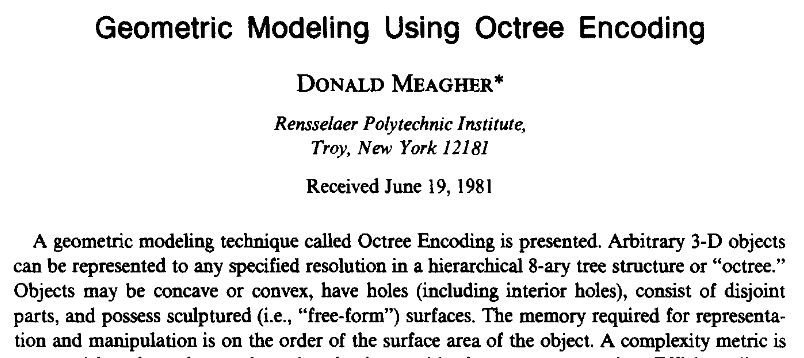
\includegraphics[width=3in]{../Pictures/octtree.png}
    \end{center}
\end{frame}

\begin{frame}[fragile]
    \frametitle{Why \texttt{deal.II}?}
    \begin{enumerate}
        \item ROMs are \emph{usually} expressed as finite element methods
        \pause
        \item Community is nice
        \pause
        \item Great documentation
    \end{enumerate}

    \pause
    \begin{center}
        {\tiny
        \begin{verbatim}
          [drwells@archway dealii-dev]$ cloc ./include
              378 text files.
              378 unique files.
              2 files ignored.

          http://cloc.sourceforge.net v 1.64  T=1.42 s (264.3 files/s, 180140.8 lines/s)
          -------------------------------------------------------------------------------
          Language                     files          blank        comment           code
          -------------------------------------------------------------------------------
          C/C++ Header                   375          34261         113105         108829
          CMake                            1              4             23             18
          -------------------------------------------------------------------------------
          SUM:                           376          34265         113128         108847
          -------------------------------------------------------------------------------
          \end{verbatim}
        }
    \end{center}
\end{frame}

\begin{frame}
    \frametitle{Why \texttt{deal.II}?}
    \begin{enumerate}
        \item LAPACK support (\texttt{geev}, \texttt{getrf}, \texttt{getrs})
        \item HDF5 and XDMF support
        \item C++11 support
    \end{enumerate}
\end{frame}

\section{Numerical Experiment}
\begin{frame}
    \frametitle{The Navier-Stokes Equations}
    \begin{equation}
        \begin{aligned}
            \vec{u}_t + \vec{u} \cdot \nabla \vec{u} - \dfrac{1}{Re} \Delta \vec{u}
            + \nabla p &= 0,                                                  \\
            \nabla \cdot \vec{u} &= 0
        \end{aligned}
    \end{equation}
    \begin{enumerate}
        \item Specified (parabolic) inflow
        \item \(\vec{u} \times \vec{n} = 0\) outflow
        \item \texttt{deal.II} step 35 \cite{dealii81, guermond05}
        \item Fractional step method
        \item About \(600,000\) DoFs, \(Re = 100\)
    \end{enumerate}
\end{frame}

\begin{frame}
    \frametitle{The Navier-Stokes Equations}
    \begin{center}
        \emph{Goal:} Preserve large structures and phase portraits.
    \end{center}
\end{frame}

\begin{frame}
    \frametitle{The Navier-Stokes Equations}
    \begin{center}
        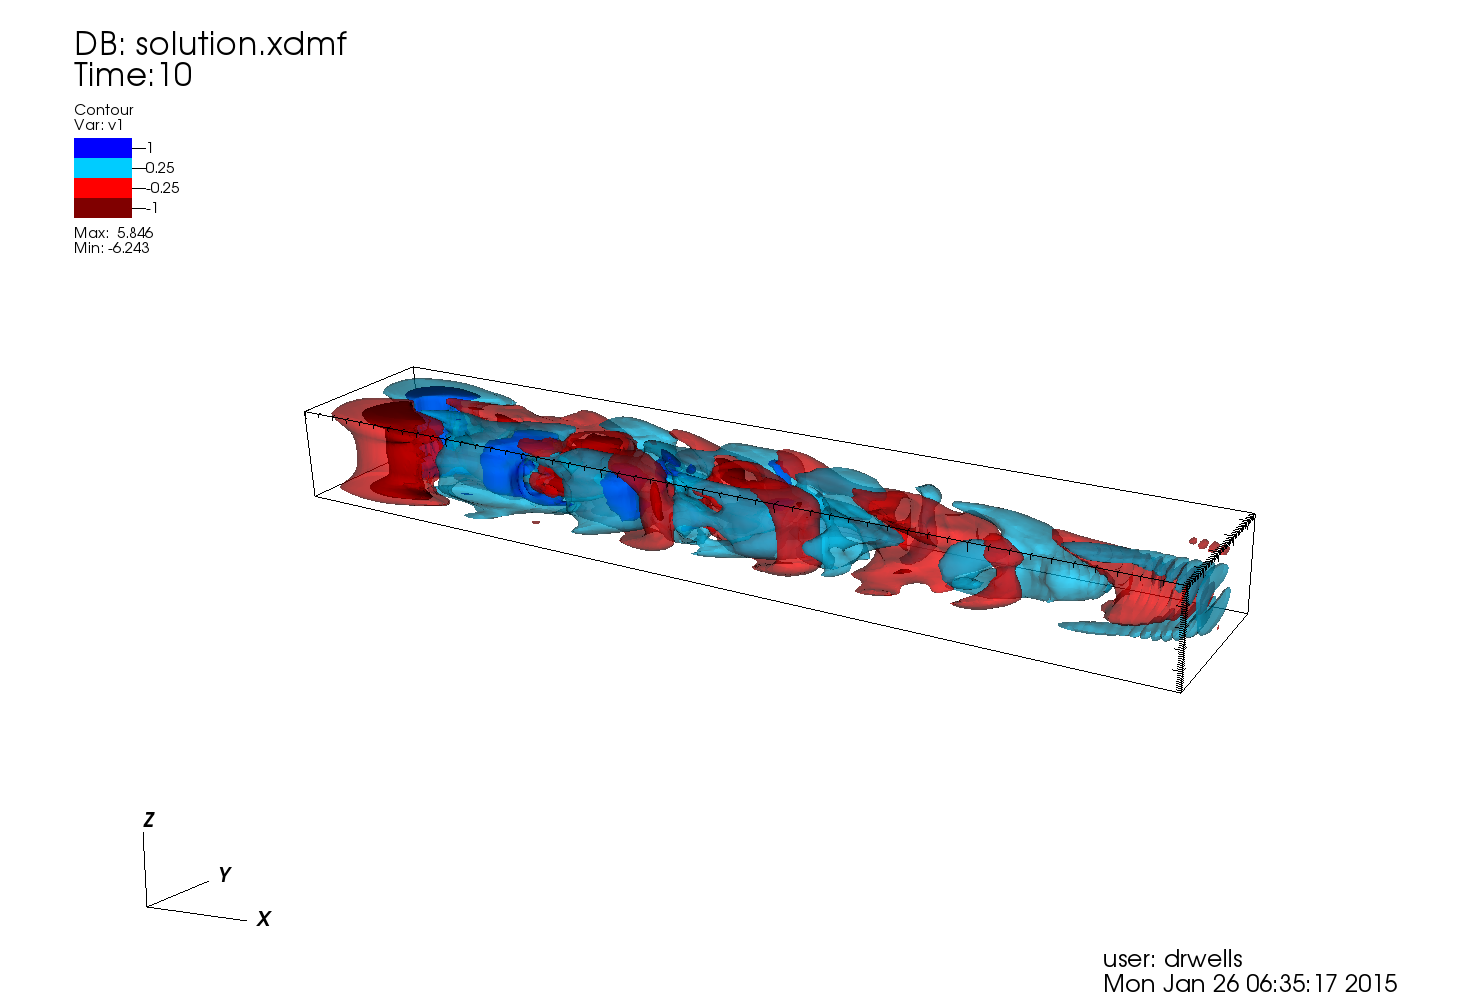
\includegraphics[width=3in]{../Pictures/NSE/ns-movie1000.png}

        \(y\)-velocity contours at \(t = 10\). There is a circular cylinder near
        the inflow on the left.
    \end{center}
\end{frame}

\section{POD}
\begin{frame}
    \frametitle{Proper Orthogonal Decomposition (POD)}
    \begin{quote}
        Given a set of data with high dimensionality, what is the best (under
        some norm) approximation to the data for a given rank \(r\)?
    \end{quote}
\end{frame}

\begin{frame}
    \frametitle{What are POD-derived basis functions?}
    Deriving POD basis functions is a linear procedure. Let \(Y\) denote the
    ``snapshot'' matrix \cite{Sir87abc} and \(M = L L^T\) denote the mass
    matrix.

    \pause
    \begin{equation}
        E S V^T = SVD(L^T Y) \rightarrow \Phi = (L^T)^{-1} E
    \end{equation}
    \pause
    \begin{equation}
        Y^T M Y \nu_i = \lambda_i \nu_i
        \rightarrow
        \varphi_i = \sum_{n = 0}^{N - 1} y_n \nu_i(n)
    \end{equation}
\end{frame}

\begin{frame}
    \frametitle{The Method of Snapshots}
    \begin{enumerate}
        \item Does either the method of snapshots or the reduced order matrices
              suffer a loss of accuracy from inaccurate inner product
              calculations?
              \pause
        \item Do the POD vectors calculated by the method of snapshots recover
              the POD interpolation error equations?
    \end{enumerate}
\end{frame}

\begin{frame}
    From \texttt{vector.templates.h}:
    \begin{center}
        {\scriptsize
          \input{c++/vector}
        }
    \end{center}
\end{frame}


\begin{frame}
    \frametitle{The Method of Snapshots}
    \begin{center}
        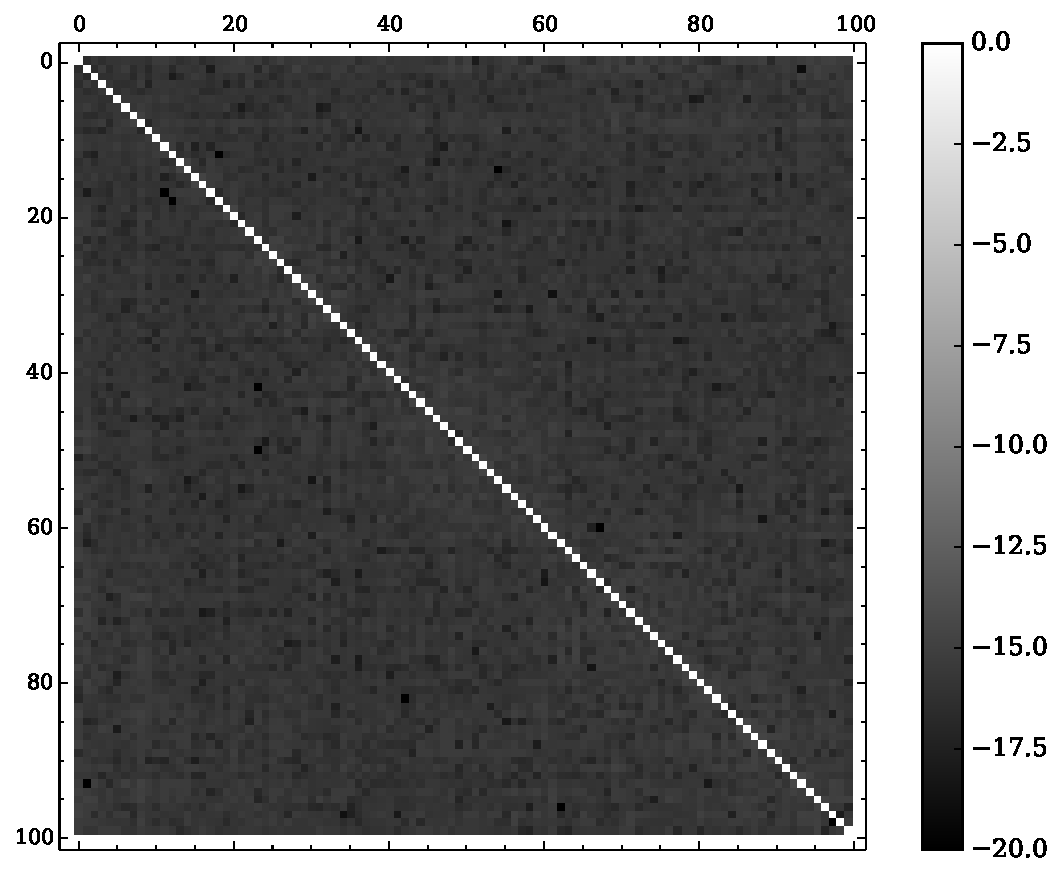
\includegraphics[width=3in]{../Pictures/POD/mass-matrix.pdf}

        Magnitudes of entries in the POD mass matrix.
    \end{center}
\end{frame}

\begin{frame}
    \frametitle{Interpolation Errors}
    \begin{figure}
        \centering
        \begin{tabular}{| l | l | l |}
            \hline
            \(r_1\) & \(\displaystyle \sum_{i = r_1}^{R - 1} \sigma_i^2\)
            & \(\displaystyle \sum_{n = 0}^{R - 1} \Norms{\uu_n - \sum_{i =
            0}^{r_1 - 1} \Langles{\uu_n, \podvec_i} \podvec_i}^2\)
                                                                              \\
            \hline
             2       &  182753.567915   &    182753.570693                    \\
             4       &  164311.705302   &    164311.712343                    \\
             6       &  156296.758264   &    156296.757146                    \\
             8       &  148780.806184   &    148780.808336                    \\
             10      &  141653.502162   &    141653.507387                    \\
             20      &  114794.313701   &    114794.326822                    \\
             40      &  83565.3337824   &    83565.3313631                    \\
             60      &  65667.1960201   &    65667.1963493                    \\
             80      &  53841.1631402   &    53841.1635371                    \\
             100     &  45045.8004678   &    45045.8035251                    \\
            \hline
        \end{tabular}
    \end{figure}
\end{frame}


\section{Filtering \& ROM}
    \begin{frame}
        \frametitle{Introduction}
        Regularized models imply the use of a filter.
    \end{frame}

    \begin{frame}
        \frametitle{The POD Projection Filter}
        For a fixed \(r_1 < r\) and a given \(\uu_r \in X^r\), the POD projection
        seeks \(\FF(\uu_r) \in X^{r_1}\) such that
        \begin{equation}
            (\FF(\uu_r), \podvec_j) = (\uu_r, \podvec_j), \forall j = 0, \cdots, r_1
            - 1.
        \end{equation}
        \pause
        Doesn't work so well, see \cite{regrompreprint}.
    \end{frame}

    \begin{frame}
        \frametitle{The POD Differential Filter}
        The POD differential filter is defined as follows: let \(\delta\) be the
        radius of the POD differential filter. For a given \(\uu_r \in X^r\),
        find \(\FF(u_r) \in X^r\) such that
        \begin{equation}
            \left((I - \delta^2 \Delta) \FF(u^r), \podvec_j\right)
            = (\uu_r, \podvec_j), \forall j = 0, \cdots, r - 1.
        \end{equation}
    \end{frame}

    \begin{frame}
        \frametitle{What does the differential filter do?}
        \begin{figure}
            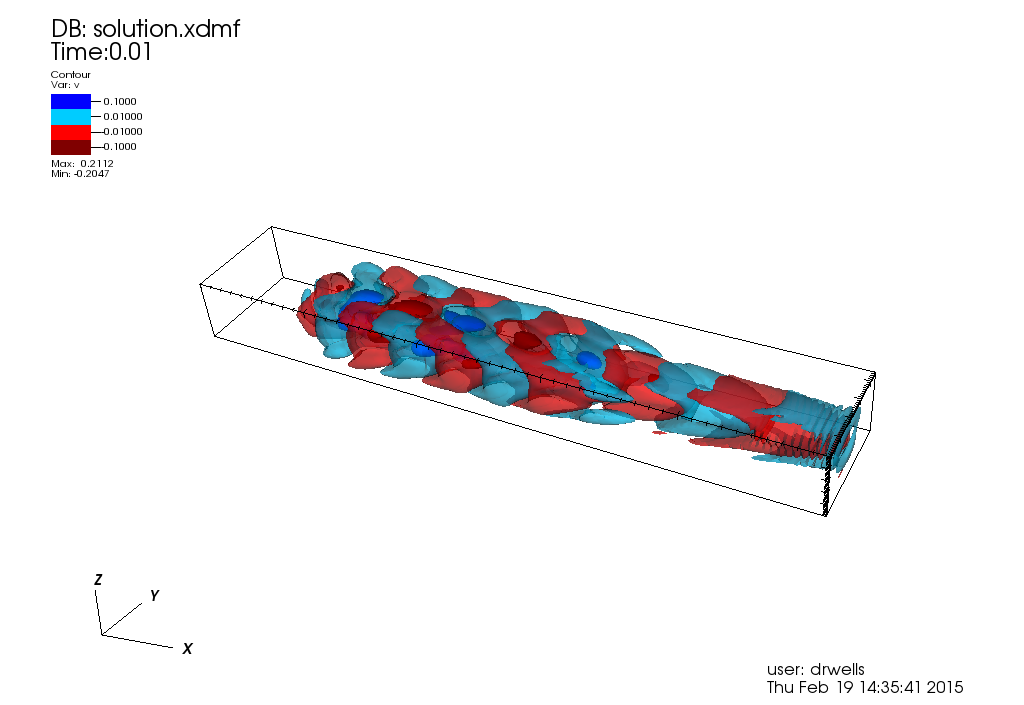
\includegraphics[width=3in]{../Pictures/NSE/pod-vector-1.png}
            \caption{The first POD vector for the NSE experiment.}
        \end{figure}
    \end{frame}

    \begin{frame}
        \frametitle{What does the differential filter do?}
        \begin{figure}
            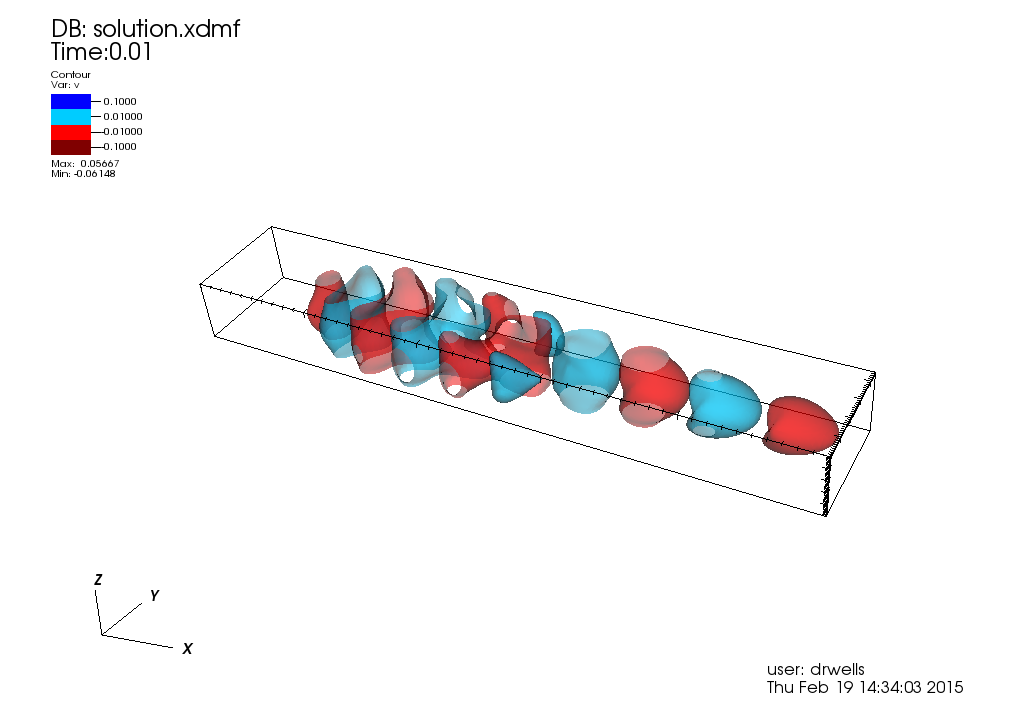
\includegraphics[width=3in]{../Pictures/NSE/filtered-pod-vector-1.png}
            \caption{The filtered first POD vector for the NSE experiment,
            $\delta = 0.5$.}
        \end{figure}
    \end{frame}

    \begin{frame}
        \frametitle{What does the differential filter do?}
        \begin{figure}
            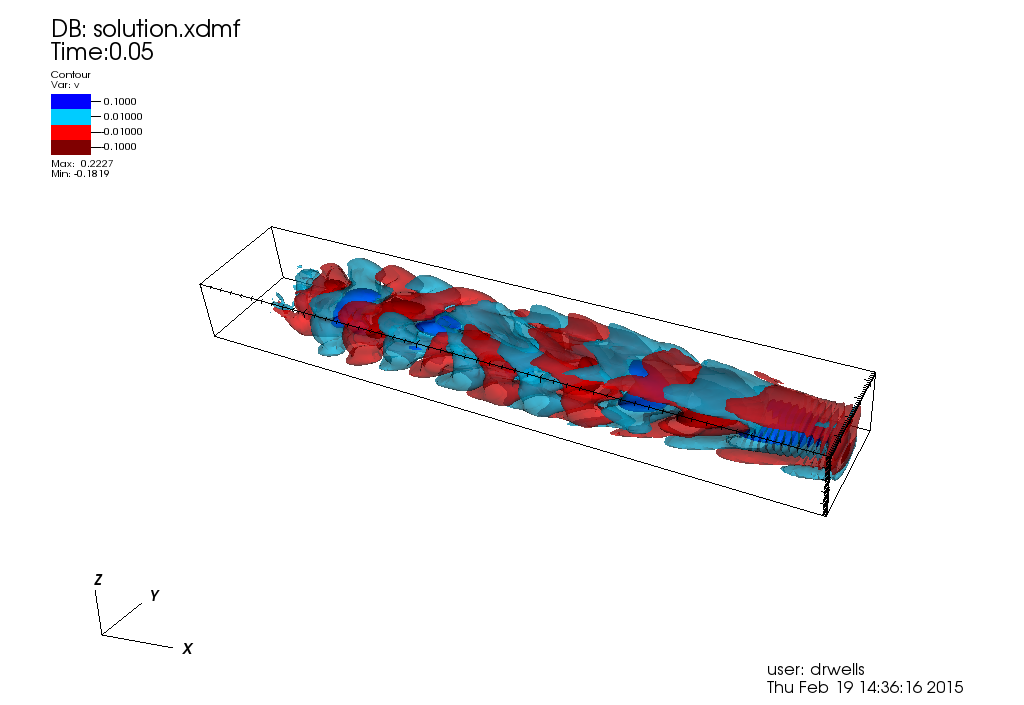
\includegraphics[width=3in]{../Pictures/NSE/pod-vector-5.png}
            \caption{The fifth POD vector for the NSE experiment.}
        \end{figure}
    \end{frame}

    \begin{frame}
        \frametitle{What does the differential filter do?}
        \begin{figure}
            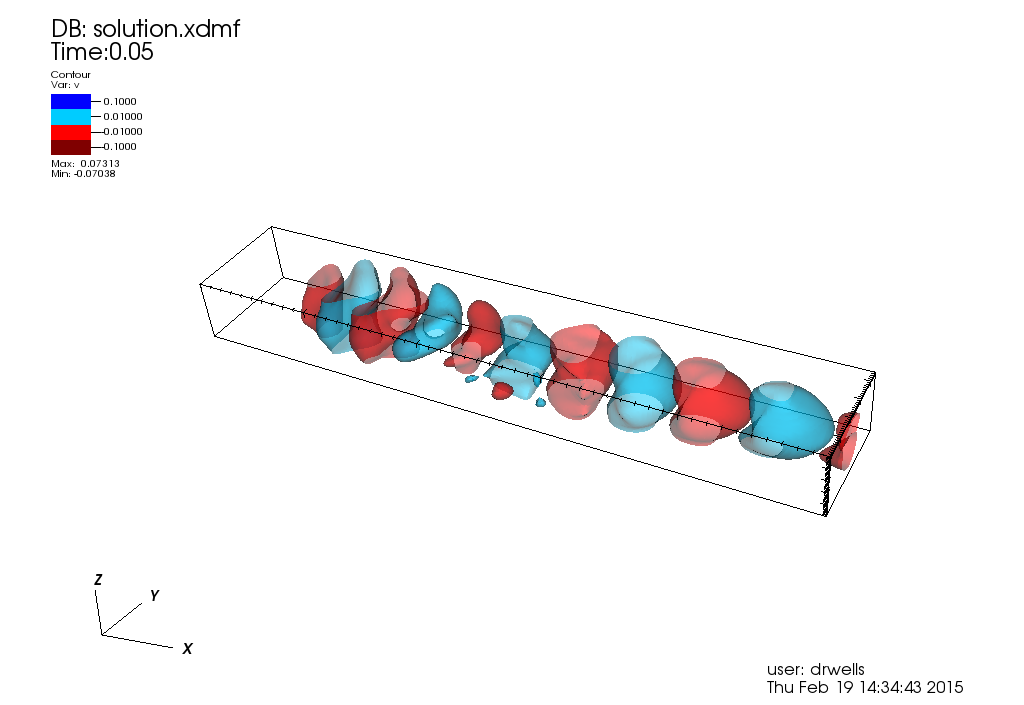
\includegraphics[width=3in]{../Pictures/NSE/filtered-pod-vector-5.png}
            \caption{The filtered fifth POD vector for the NSE experiment,
            $\delta = 0.5$.}
        \end{figure}
    \end{frame}

\section{REG-ROMs}
\begin{frame}
    \frametitle{Overview}
    Considered REG-ROMs:
    \begin{enumerate}
        \item Leray regularization \cite{leray1934}
        \item Evolve-then-filter \cite{LaytonADBook}
    \end{enumerate}
    \pause
    REG-ROMs are not:
    \begin{enumerate}
        \item consistent with the original PDE
        %% TODO more here
    \end{enumerate}
\end{frame}

\begin{frame}
    \frametitle{The Navier-Stokes ROM}
    For \(\uu \approx \uu_s + \uu_r\):
    \begin{equation}
        \begin{aligned}
            (\podvec_i, \uu_{r,t})
            &= -\dfrac{1}{Re} (\nabla \podvec_i, \nabla (\uu_s + \uu_r))
            + \dfrac{1}{Re} \int_{\Gamma_2} \podvec_i[0] u_{x}[0] dl          \\
            &- (\podvec_i, (\uu_s + \uu_r) \cdot \nabla (\uu_s + \uu_r))
        \end{aligned}
    \end{equation}

    Combination of linear \((r \times r)\), quadratic \((r \times r \times r)\),
    and constant \((r \times 1)\) terms.
    \pause
    \emph{Goal:} only change computational complexity by at most \(\OO(r^2)\).
\end{frame}

\begin{frame}
    \frametitle{The Leray Regularization} Jean Leray, 1934 \cite{leray1934}:
    existence of solutions (modulo a subsequence) to the \emph{regularized}
    Navier-Stokes equations
    \begin{equation}
        \vec{u}_t - \dfrac{1}{Re} \Delta \vec{u}
        + \mathcal{F}(\vec{u}) \cdot \nabla \vec{u}
        + \nabla p = 0
    \end{equation}

    We rewrite the nonlinearity in the ROM as
    \begin{equation}
        \int_\Omega \vec{\varphi}_i \cdot
        (\vec{\varphi}_j \cdot \nabla \vec{\varphi}_k) \,dx
        \rightarrow
        \int_\Omega \vec{\varphi}_i \cdot
        (\mathcal{F}(\vec{\varphi}_j) \cdot \nabla \vec{\varphi}_k) \,dx
    \end{equation}
\end{frame}

\begin{frame}
    \begin{center}
        {
        \scriptsize
        \input{c++/rk_factory}
        }
    \end{center}
    \pause

    Use \texttt{unique\_ptr} to implement factories and assemble the correct
    regularized model. \pause No need for \texttt{delete}.
\end{frame}

\begin{frame}
    \frametitle{What happens as we vary \(\delta\)?}
    \begin{figure}
        \centering
        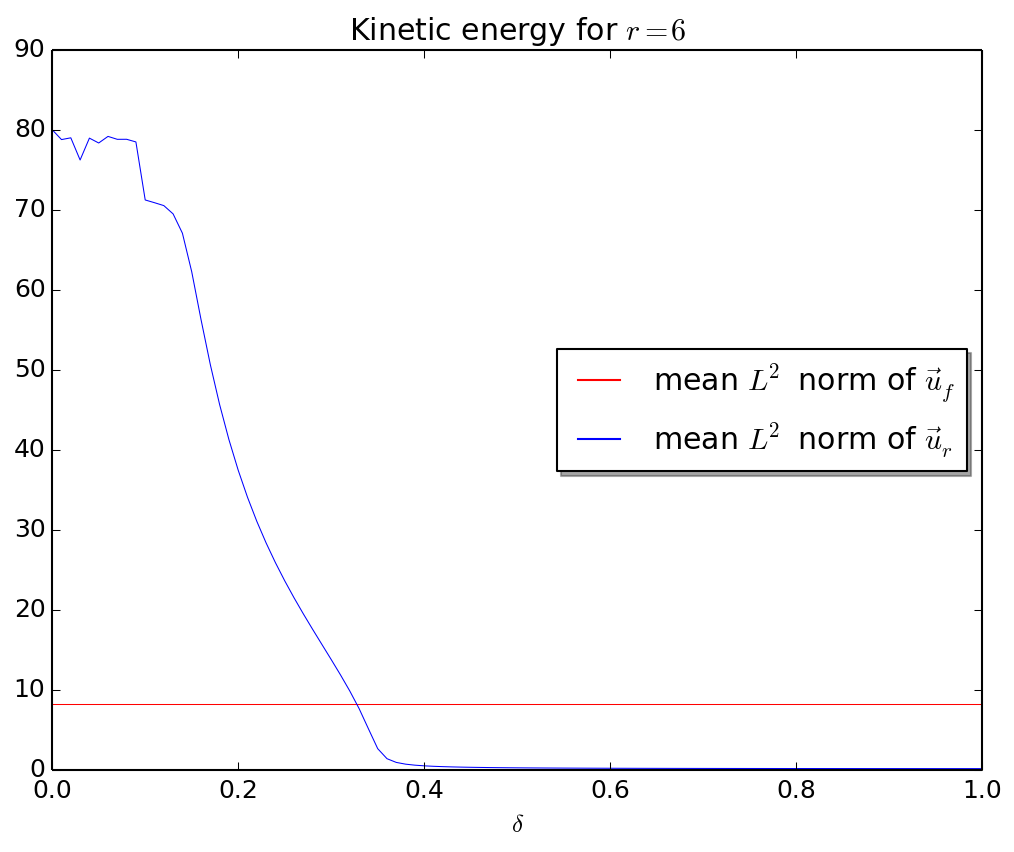
\includegraphics[width=3in]{../Pictures/NSE/leray-df/r-6/mean-ke.png}

        The effect of \(\delta\) (\(x\)-axis) on the mean kinetic energy
        (\(y\)-axis), with the correct mean in red and the Leray-DF-ROM in blue.
    \end{figure}
\end{frame}

\begin{frame}
    \frametitle{What happens as we vary \(\delta\)?}
    \begin{figure}
        \centering
        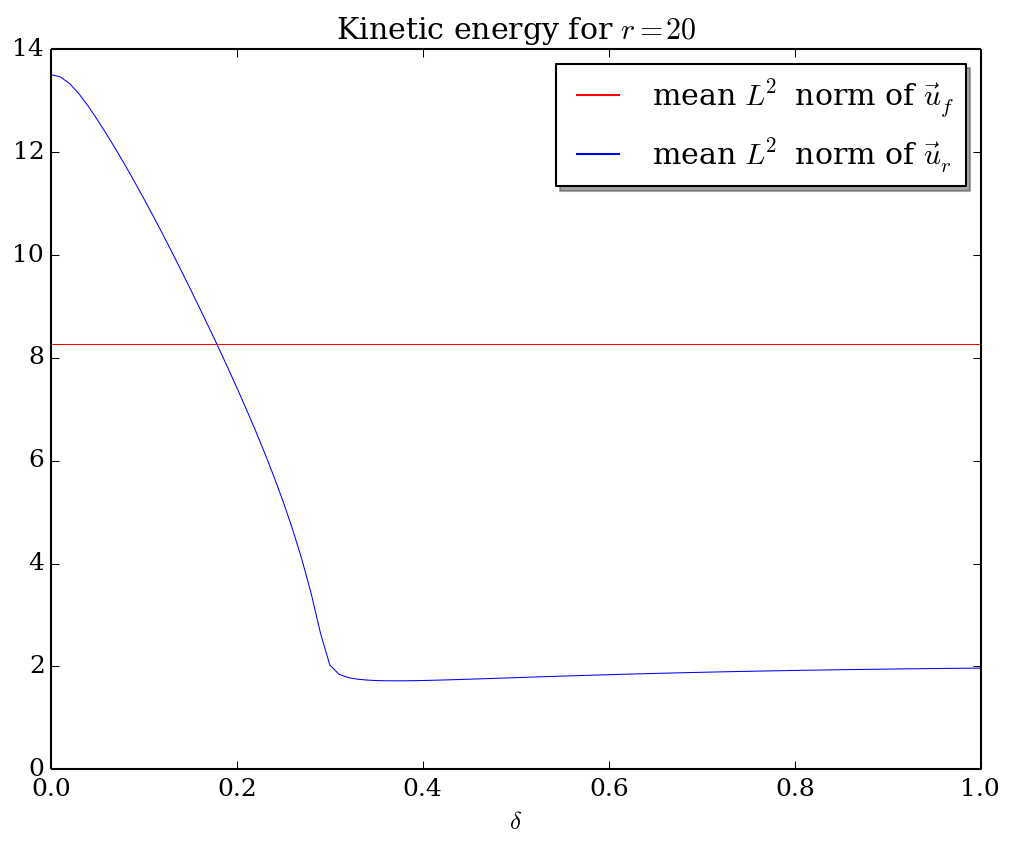
\includegraphics[width=3in]{../Pictures/NSE/leray-df/r-20/mean-ke.png}

        The effect of \(\delta\) (\(x\)-axis) on the mean kinetic energy
        (\(y\)-axis), with the correct mean in red and the Leray-DF-ROM in blue.
    \end{figure}
\end{frame}

\begin{frame}
    \frametitle{What is the optimal value for \(\delta\)?}
    \begin{figure}
        \centering
        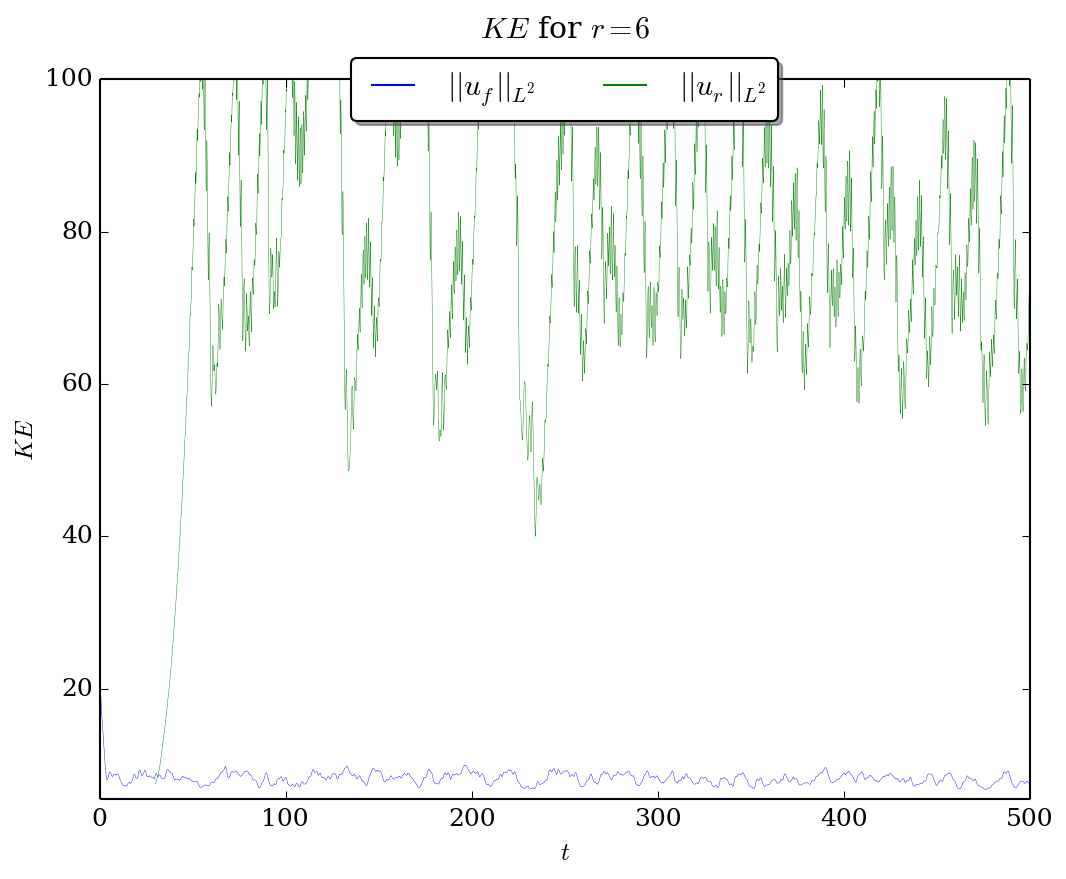
\includegraphics[width=3in]{../Pictures/NSE/galerkin/r-6/ke.png}

        \caption{Galerkin ROM (\(r = 6\)), in green, with the DNS in blue.}
    \end{figure}
\end{frame}

\begin{frame}
    \frametitle{What is the optimal value for \(\delta\)?}
    \begin{figure}
        \centering
        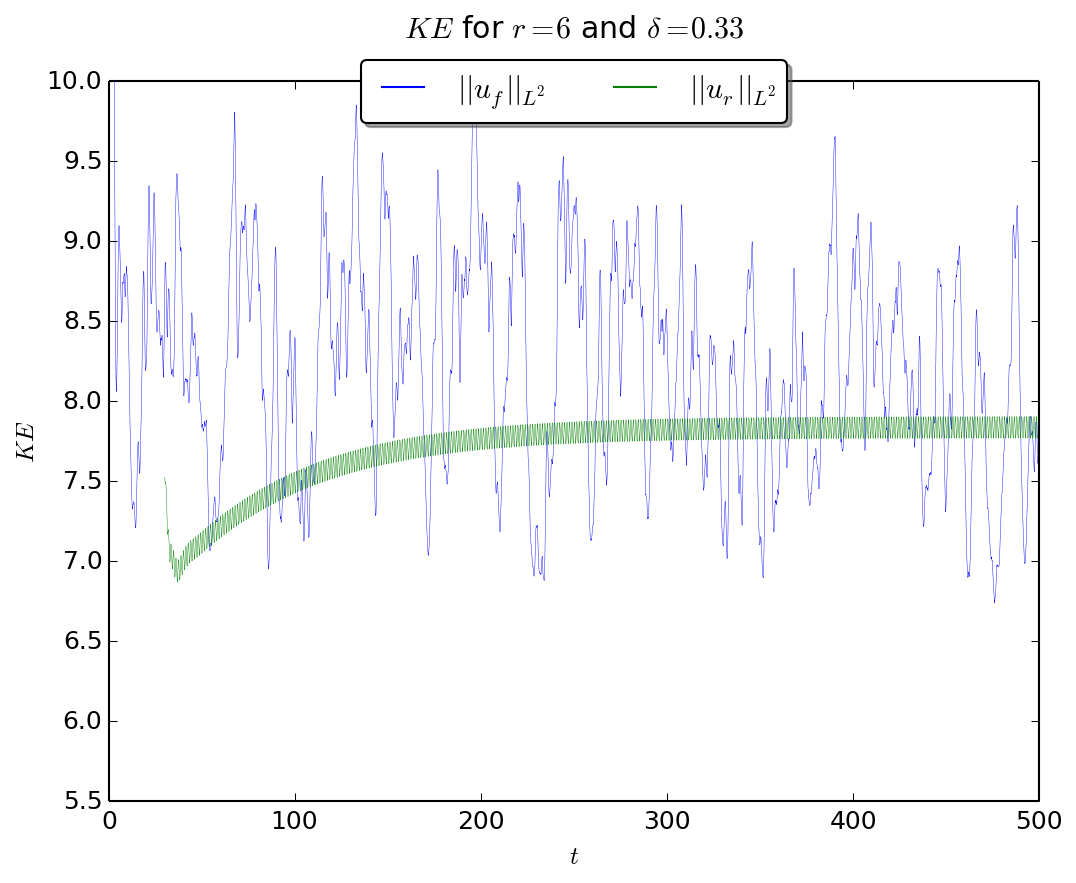
\includegraphics[width=3in]{{../Pictures/NSE/leray-df/r-6/ke-delta-0.33}.png}

        \caption{POD-ROM with $\delta = 0.33$, green.}
    \end{figure}
\end{frame}

\begin{frame}
    \frametitle{What is the optimal value for \(\delta\)?}
    \begin{figure}
        \centering
        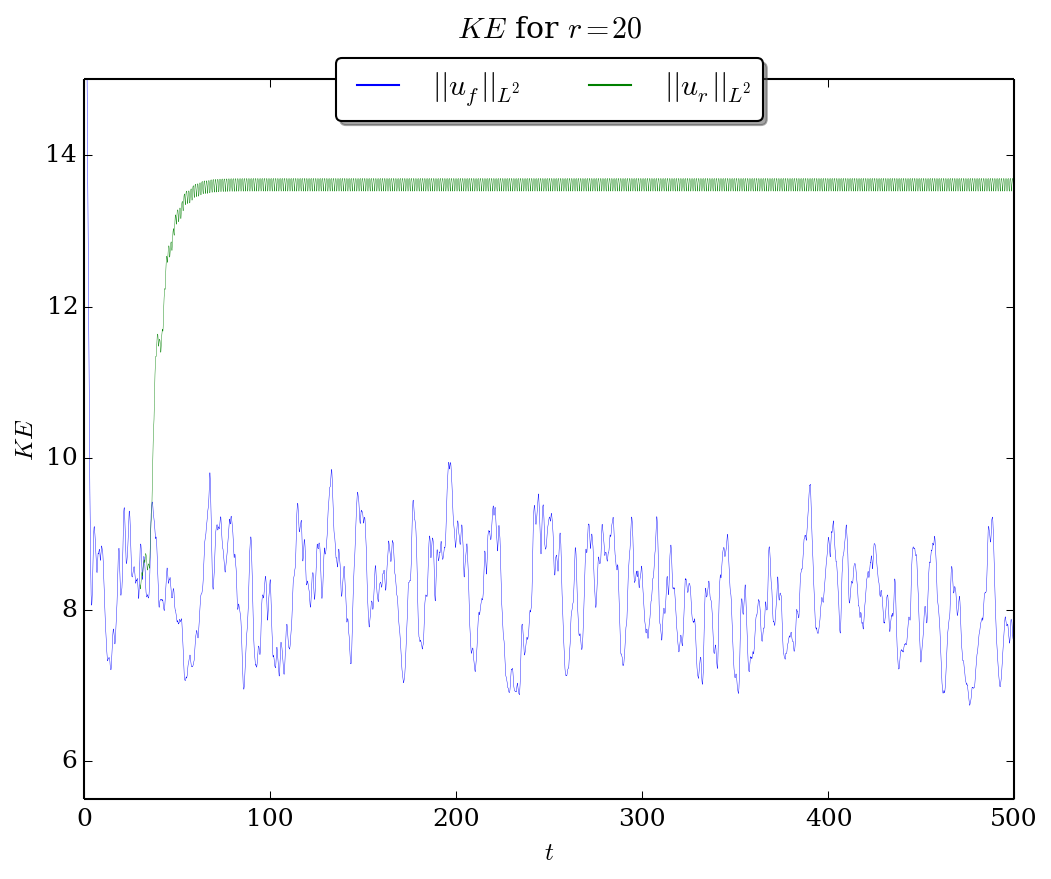
\includegraphics[width=3in]{../Pictures/NSE/galerkin/r-20/ke.png}

        \caption{Galerkin ROM (\(r = 20\)), in green, with the DNS in blue.}
    \end{figure}
\end{frame}

\begin{frame}
    \frametitle{What is the optimal value for \(\delta\)?}
    \begin{figure}
        \centering
        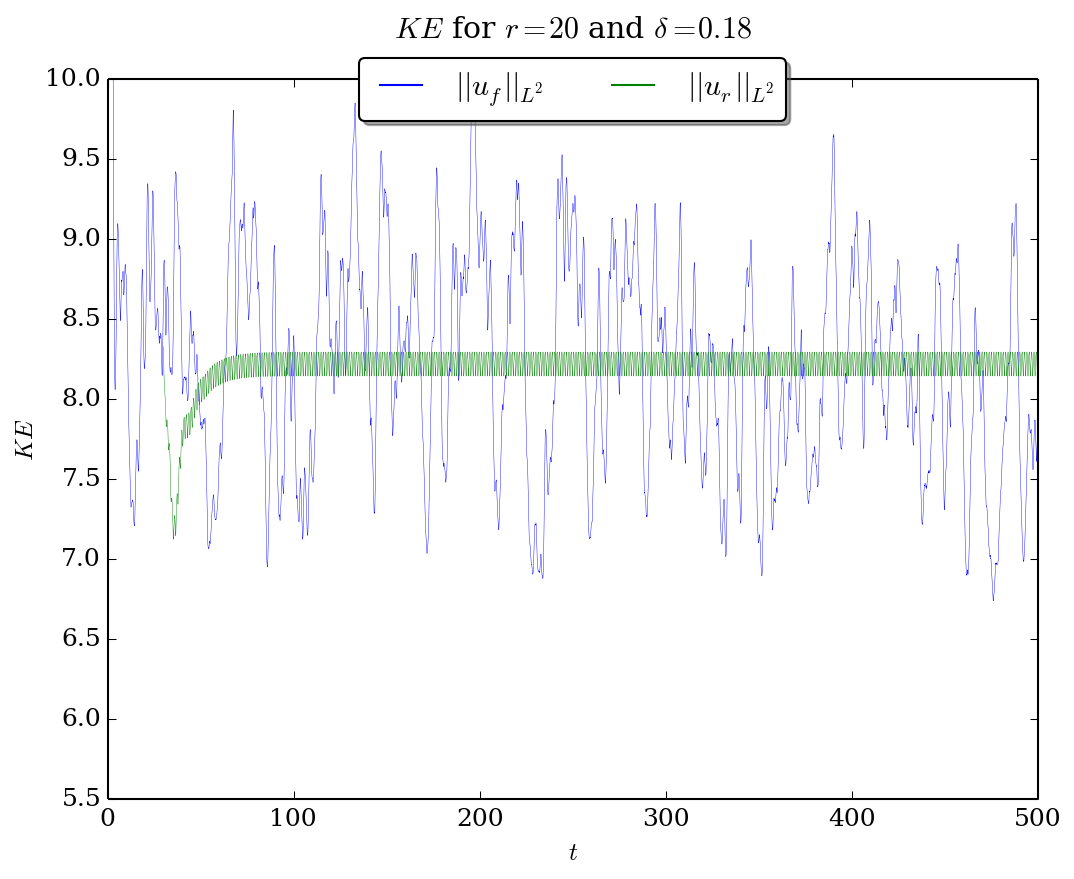
\includegraphics[width=3in]{{../Pictures/NSE/leray-df/r-20/ke-delta-0.18}.png}

        \caption{POD-ROM with $\delta = 0.18$, green.}
    \end{figure}
\end{frame}

\begin{frame}
    \frametitle{Does changing \(\delta\) ``fix'' the phase plots?}
    Yes!
    \begin{figure}
        \centering
        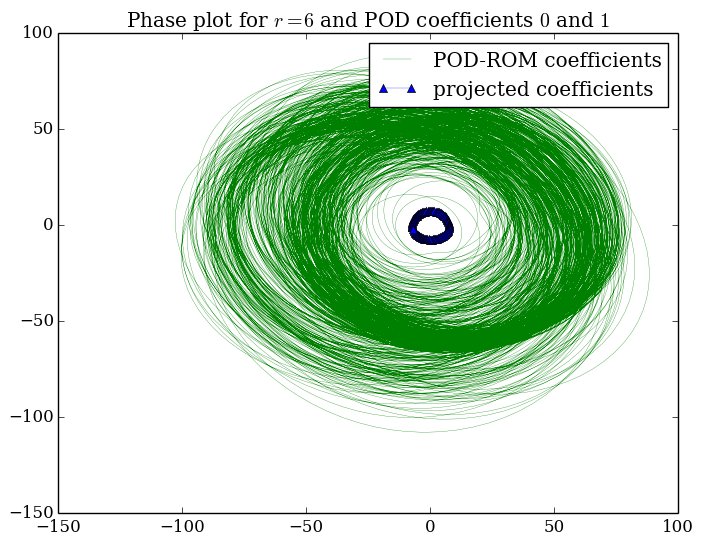
\includegraphics[width=3in]{../Pictures/NSE/galerkin/r-6/phase-0-1.png}

        Phase plot for the first and second POD vectors with \(\delta = 0\).
    \end{figure}
\end{frame}

\begin{frame}
    \frametitle{Does changing \(\delta\) ``fix'' the phase plots?}
    Yes!
    \begin{figure}
        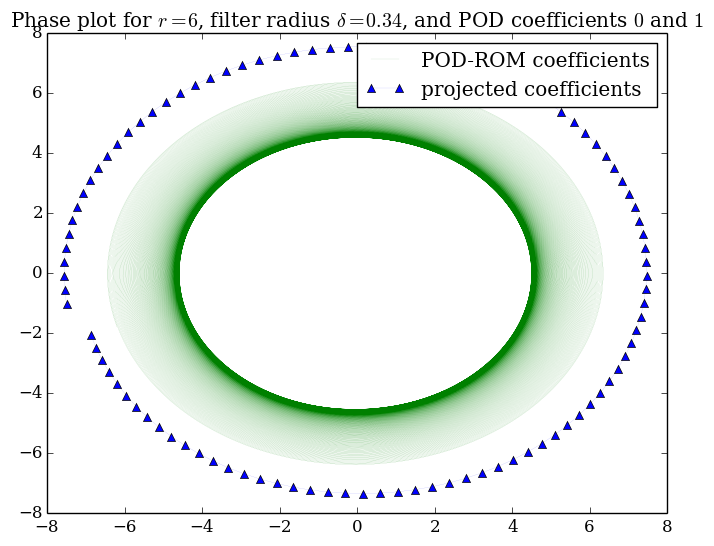
\includegraphics[width=3in]{{../Pictures/NSE/leray-df/r-6/phase-radius-0.34-0-1}.png}

        Phase plot for the first and third POD vectors with \(\delta = 0.34\).
    \end{figure}
\end{frame}

\begin{frame}
    \frametitle{Does changing \(\delta\) ``fix'' the phase plots?}
    Yes!
    \begin{figure}
        \centering
        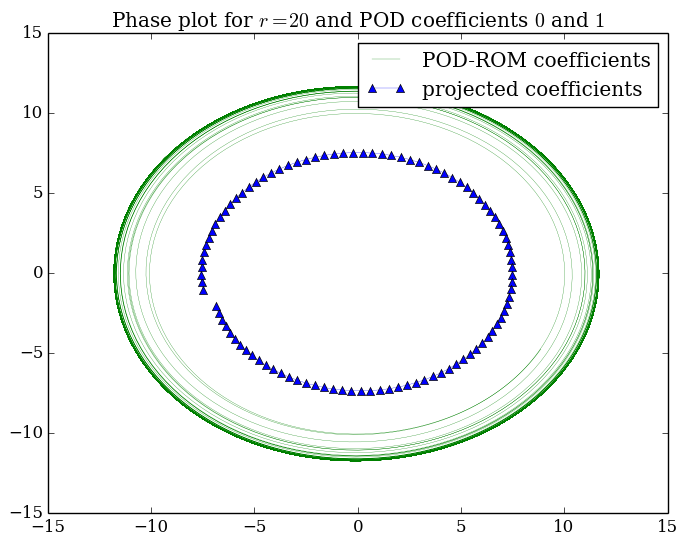
\includegraphics[width=3in]{../Pictures/NSE/galerkin/r-20/phase-0-1.png}

        Phase plot for the first and second POD vectors with \(\delta = 0\).
    \end{figure}
\end{frame}

\begin{frame}
    \frametitle{Does changing \(\delta\) ``fix'' the phase plots?}
    Yes!
    \begin{figure}
        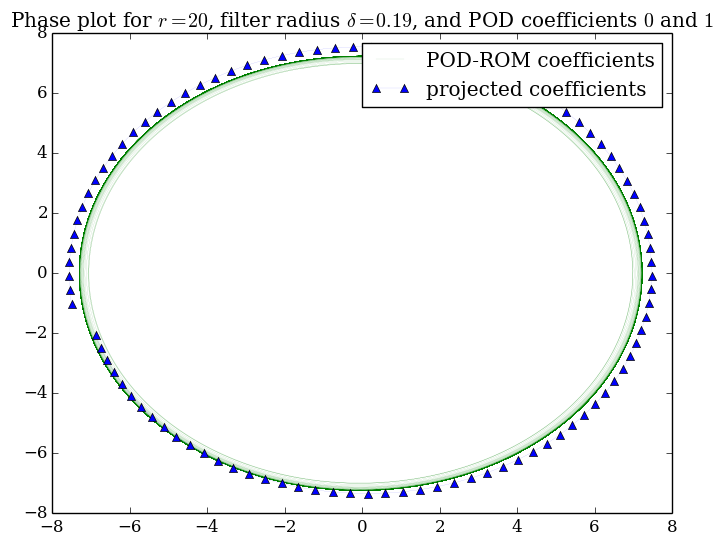
\includegraphics[width=3in]{{../Pictures/NSE/leray-df/r-20/phase-radius-0.19-0-1}.png}

        Phase plot for the first and third POD vectors with \(\delta = 0.34\).
    \end{figure}
\end{frame}


\begin{frame}
    \frametitle{An Evolve-And-Filter Model}
    Evolve:
    \begin{equation}
        \begin{aligned}
            \left(\dfrac{\ww_r^{n + 1} - \uu_r^{n + 1}}{\Delta t}\right)
            &+ \dfrac{1}{Re} \left(\nabla \uu_s + \uu_r^n, \nabla
            \podvec_k\right)                                                  \\
            &+ \left(((\uu_s + \uu_r^n) \cdot \nabla) (\uu_s + \uu_r^n),
            \podvec_k\right)
            = 0,                                                              \\
        \end{aligned}
    \end{equation}
    then filter:
    \begin{equation}
        \uu_r^{n + 1} = \FF(\ww_r^{n + 1}).
    \end{equation}
    \pause
    In practice, I use RK4 instead of forward Euler.
\end{frame}

\begin{frame}
    \frametitle{An Evolve-And-Filter Model}
    For the differential filter:
    \begin{figure}
        \centering
        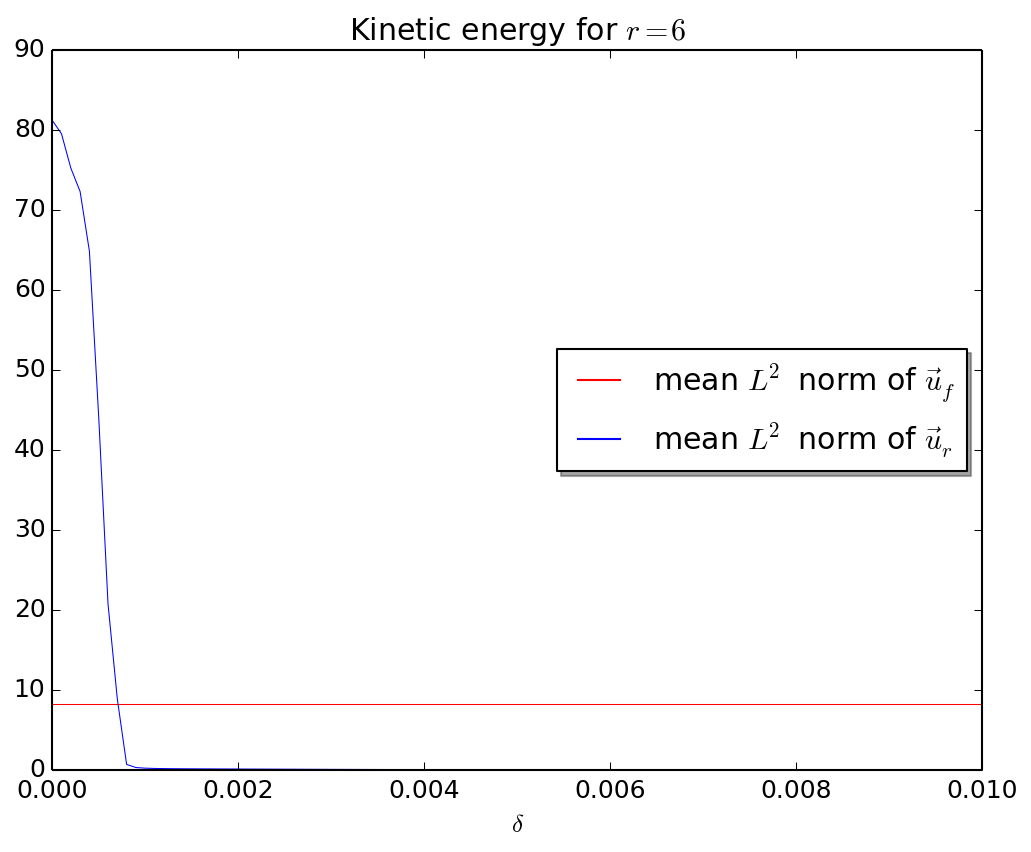
\includegraphics[width=3in]{../Pictures/NSE/ef-df/r-6/mean-ke.png}

        \caption{Mean kinetic energy based on filter radius.}
    \end{figure}
\end{frame}

\begin{frame}
    \frametitle{An Evolve-And-Filter Model}
    For the differential filter:
    \begin{figure}
        \centering
        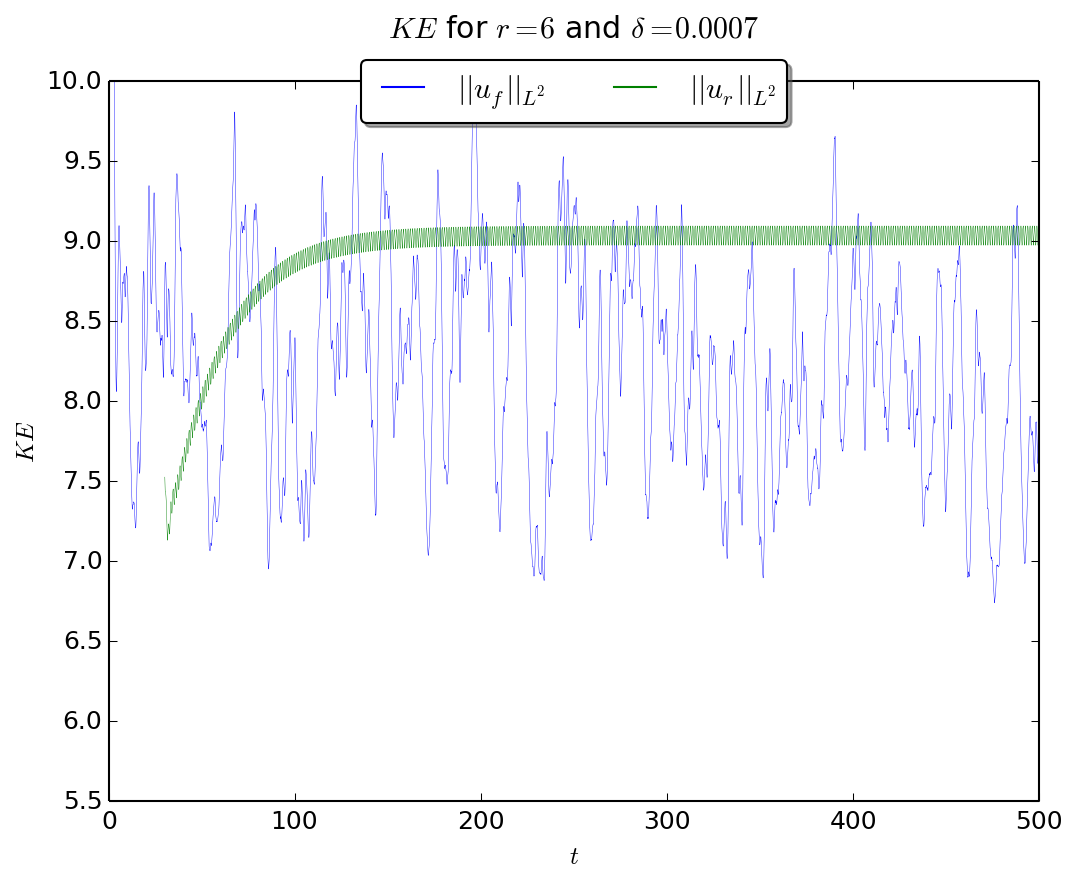
\includegraphics[width=3in]{{../Pictures/NSE/ef-df/r-6/ke-delta-0.0007}.png}

        \caption{A slight overshoot: \(\delta = 0.0007\).}
    \end{figure}
\end{frame}

\begin{frame}
    \frametitle{An Evolve-And-Filter Model}
    For the differential filter:
    \begin{figure}
        \centering
        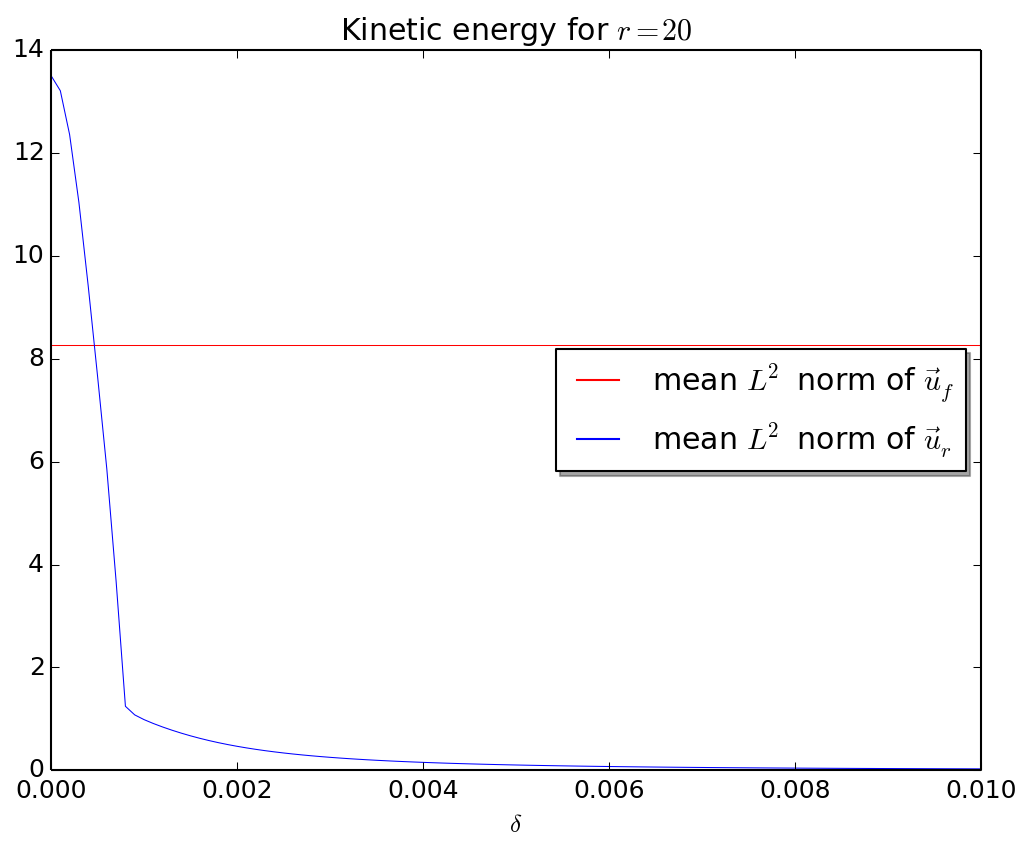
\includegraphics[width=3in]{../Pictures/NSE/ef-df/r-20/mean-ke.png}

        \caption{Mean kinetic energy based on filter radius.}
    \end{figure}
\end{frame}

\begin{frame}
    \frametitle{An Evolve-And-Filter Model}
    For the differential filter:
    \begin{figure}
        \centering
        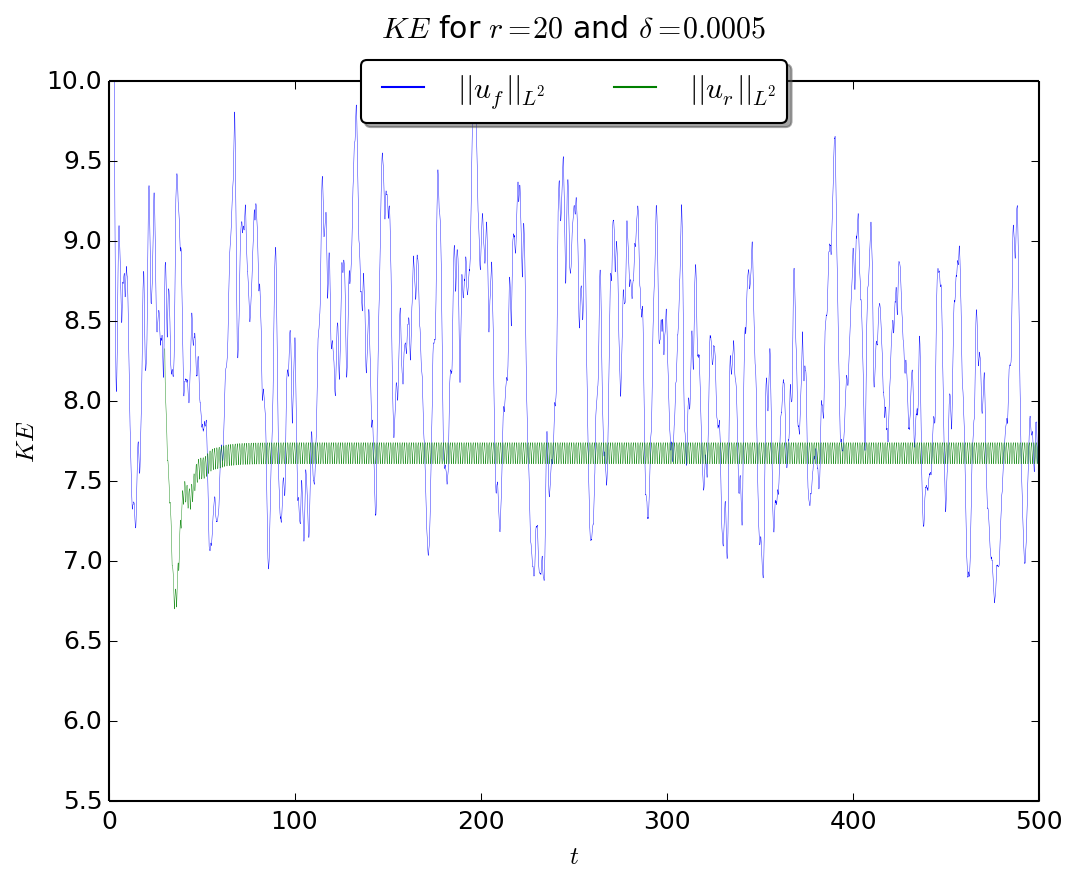
\includegraphics[width=3in]{{../Pictures/NSE/ef-df/r-20/ke-delta-0.0005}.png}

        \caption{Kinetic energy over time for \(\delta = 0.0005\).}
    \end{figure}
\end{frame}

\section{Conclusions}
    \begin{frame}
        \frametitle{Conclusions}
        \begin{enumerate}
            \item Stabilization and regularization techniques can work for ROM.
            \item Can ROM predict large structures? Sometimes.
        \end{enumerate}
    \end{frame}

    \begin{frame}
        \frametitle{Future Work: Big ROM Questions}
        \begin{enumerate}
            \item Can ROMs predict large structures correctly?
            \item Where do ROMs currently fail?
            \item Does the energy cascade apply to POD-ROMs?
            \item Can we justify this rigorously?
        \end{enumerate}
    \end{frame}

    \begin{frame}
        \frametitle{Future Work: Regularization}
        \begin{enumerate}
            \item Are there better filtering models?
            \pause
            \item Deconvolution is an easy improvement to the Leray model.
        \end{enumerate}
    \end{frame}

    \begin{frame}
        %This is the standard bibtex file
        %uncomment the following to include your bibliography
        \bibliographystyle{plain}
        \tiny
        {
        \bibliography{../thesis.bib}
        }
    \end{frame}
\end{document}
